\documentclass[12pt]{article}
%\documentstyle[12pt,aaspp4,epsf,flushrt,textpos,graphicx,hyperref,fancyhdr]{article}

\usepackage{aaspp4}
\usepackage{flushrt}
\usepackage{graphicx}

%\slugcomment {{\bf Technical Instrument Report WFC3 2014-XXX}}

\def\ssection#1{\section{\hbox to \hsize{\large\bf #1\hfill}}}
\def\ssectionstar#1{\section*{\hbox to \hsize{\large\bf #1\hfill}}}
\def\ssubsection#1{\subsection{\hbox to \hsize{#1\hfill}}}
\def\ssubsubsection#1{\subsubsection{\hbox to \hsize{#1\hfill}}}
\def\ssubsectionstar#1{\subsection*{\hbox to \hsize{#1\hfill}}}

\usepackage{hyperref}
\usepackage{breqn}
\usepackage{listings}
\usepackage{color}
\usepackage[utf8]{inputenc}

%%% GBB cute but chokes my pdflatex and the GitHub version
% Stuff for neato watermark.
% \usepackage[printwatermark]{xwatermark}
% \usepackage{xcolor,tikz}
% \newsavebox\draftbox
% \savebox\draftbox{\tikz[color=red,opacity=0.1]\node{DRAFT};}
% \newsavebox\datebox
% \savebox\datebox{\tikz[color=red,opacity=0.1]\node{\today};}
% \newwatermark*[
%   allpages,
%   angle=52.31,    % = arctan(11./8.5)
%   scale=6,
%   xpos=-35,
%   ypos=40
% ]{\usebox\draftbox\\[-30pt] \usebox\datebox}

\usepackage{fancyhdr}
\usepackage[us,12hr]{datetime} % `us' makes \today behave as usual in TeX/LaTeX
\fancypagestyle{plain}{
\fancyhf{}
\rhead{{\it Draft: {\ddmmyyyydate\today} at \currenttime}}
\lhead{{Technical Instrument Report WFC3 2014-XXX}}
\cfoot{-- \thepage\ --}
\renewcommand{\headrulewidth}{0pt}}
\pagestyle{plain}

\usepackage{enumitem}
\setlist{itemsep=0pt, topsep=0pt}
%\setlist[description]{itemsep=0pt, parsep=0pt}

\definecolor{codegreen}{rgb}{0,0.6,0}
\definecolor{codegray}{rgb}{0.5,0.5,0.5}
\definecolor{codepurple}{rgb}{0.58,0,0.82}
\definecolor{backcolour}{rgb}{0.98,0.98,0.98}
 
\lstdefinestyle{mystyle}{
    backgroundcolor=\color{backcolour},   
    commentstyle=\color{codegreen},
    keywordstyle=\color{magenta},
    numberstyle=\tiny\color{codegray},
    stringstyle=\color{codepurple},
    basicstyle=\ttfamily\footnotesize,
    breakatwhitespace=false,         
    breaklines=true,                 
    captionpos=b,                    
    keepspaces=true,                 
    numbers=left,                    
    numbersep=5pt,                  
    showspaces=false,                
    showstringspaces=false,
    showtabs=false,                  
    tabsize=2
}
 
\lstset{style=mystyle}
\hypersetup{colorlinks=true}

\long\def\symbolfootnote[#1]#2{\begingroup%
  \def\thefootnote{\fnsymbol{footnote}}\footnote[#1]{#2}\endgroup%
  \def\footnoterule{\null}}

\def\normalfootnote#1{\def\footnoterule{\kern 40pt\hrule width 2truein \kern 2.4pt}\footnote{#1}}

%%%%%%%%%%%%%%%%%%%%%
% Title and authors
%%%%%%%%%%%%%%%%%%%%%

\begin{document}

%\null \vskip-2.76truecm \hskip-0.84truecm
\null \vskip-6.25truecm \hskip-0.84truecm
%\epsfxsize=5.truecm %size to play with
%\epsfbox{stlogoplus.eps}

\includegraphics[width=5.7truecm, angle=0.0]{stlogoplus.pdf}

\title{\Huge
\hbox to \hsize{\hfill \bf Current \textit{HST} Slitless}}
\vskip-0.8truecm
\affil{\Huge \hbox to \hsize{\hfill \bf Spectroscopy Simulation Software}}

\vskip-1.4truecm
\hbox to \hsize{\hfill \hbox to 5truecm{\hrulefill}}

\medskip

\author{\hbox to \hsize{\hfill STScI WFC3 Grism Group: G. Brammer, N. Pirzkal, R. E. Ryan}}
%\author{\hbox to \hsize{\hfill G. Brammer, N. Pirzkal, R. E. Ryan}}

% \vskip-0.5truecm
% \affil{\hbox to \hsize{\hfill }}
%\vskip-0.5truecm
\affil{\hbox to \hsize{\hfill Draft version: \today}}

\vskip-0.3truecm

%%%%%%%%%%%%%%%
% Abstract
%%%%%%%%%%%%%%%

\hrule height 1.5pt
\smallskip
\noindent \large{\bf A}\footnotesize{\bf BSTRACT}

\noindent\normalsize{\textit{We describe the properties of three independently-developed software packages used to simulate slitless spectroscopic data from the Hubble Space Telescope.  The first, \texttt{aXe}/\texttt{aXeSIM}, was developed by the ST-ECF for ACS and later adapted for use with NICMOS and WFC3 data,  and is officially supported by STScI for the \textit{HST} user community.  The other two packages were developed for personal use by N. Pirzkal and by G. Brammer.  In this document we describe and compare the capabilities, key assumptions, outputs and runtime of the three separate software packages, which define the current state-of-the art for the analysis of space-based slitless spectroscopic data.}}

\smallskip
\medskip
\hrule height 1.5pt

\symbolfootnote[0]{Copyright {\copyright} 2014 The Association of
  Universities for Research in Astronomy, Inc. All Rights Reserved.}

%\begin{document}

%\title{Current \textit{HST} Slitless Spectroscopy Simulation Software}

% Note: This document is from the WFC3 team, specifically from the people workign on grism in WFC3.
%\author{STScI WFC3 Grism Group \\ (G. Brammer, N. Pirzkal, R. E. Ryan)}

% \begin{abstract}
%     We describe the properties of three independently-developed software packages used to simulate slitless spectroscopic data from the Hubble Space Telescope.  The first, \texttt{aXe}/\texttt{aXeSIM}, was developed by the ST-ECF for ACS and later adapted for use with NICMOS and WFC3 data,  and is officially supported by STScI for the \textit{HST} user community.  The other two packages were developed for personal use by N. Pirzkal and by G. Brammer.  In this document we describe and compare the capabilities, key assumptions, outputs and runtime of the three separate software packages, which define the current state-of-the art for the analysis of space-based slitless spectroscopic data.
%     
% \end{abstract}

% \textit{Draft version: \today}\footnote{For updates to this document, see
% \url{https://github.com/WFC3Grism/CodeDescription/}}.

% N. Pirzkal, R. E. Ryan
\ssection{Grism data}

% RER: I would write it like this...

Grism observations are obtained by inserting a dispersive element in the light path.  In normal imaging mode, the detector provides a pixelized sampling of some scene:
\begin{dmath}
I(x,y) = \int f(x,y,\lambda)\,\mathcal{S}(\lambda)\,d\lambda
\end{dmath}
where $I(x,y)$ refers to the direct image, $f(x,y,\lambda)$ is intrinsic spectrum at each pixel in the scene, and $\mathcal{S}(\lambda)$ is the sensitivity curve (which in principle depends on detector position as well). The dispersive element transforms $f(x,y,\lambda)$ by redistributing the $\lambda$ dimension.  As described below, this transformation is field-dependent and can be encoded in a series of spatially-varying polynomials that have been calibrated for both WFC3 and ACS.

In the slitless case, the disperser defines a spectral trace, essentially mapping a given wavelength $\lambda$\ onto a unique $x'$,$y'$\ position on the detector. Such a trace is shown in Figure \ref{fig:1}. Assuming no change in sensitivity as a function of position, and ignoring pixel flat-fielding, a dispersed image can be thought of a the convolution of the direct image with the spectra trace:
\begin{dmath}
G(x,y) =  f(x,y,\lambda) \otimes tr(\lambda).
\end{dmath}

\begin{figure}[!t]
\centering
\includegraphics[width=\textwidth]{"Figures/Grism_Equation"}
\caption{A simplified view of the relation between the information provided by the direct image (left), the transfer function of the dispersive element, the trace (middle), and the convolution of the two. If one ignores flat-fielding and wavelength dependence of the shape of the object, this can be considered (and simulated using) a 2D convolution.}
\label{fig:1}
\end{figure}

Slitless grism observations can therefore be simulated starting from a set of direct images, which provide information about the field and the objects within it, and sufficient understanding of the properties of the dispersing element.
All of the existing analysis software we describe below currently rely on a set of direct observations of the field, or at least a catalog of objects, complete with their size and brightness. 

\ssection{Contamination}
Contamination is a drawback of slitless spectroscopy. First, the lack of slits results in the subtle effect that the effective resolution of the disperser is lowered by the size of the footprint of the objects along the dispersion direction. Hence, a larger object will produce a spectrum that is smoothed out. This is visible in Figure \ref{fig:1} where we show that the leftmost and rightmost pixels of the source, shown on the left of the figure, are projected onto the same sets of pixels on the right-hand side of the Figure. This self contamination depends on the direction of the dispersion and orientation of the source. A non-symmetrical source will therefore produce spectra of different effective resolution at different position angles on the sky. Second, spectra of neighboring objects can contaminate one another and this is again sensitive to the orientation at which the data are obtained. Figure \ref{fig:2} illustrates this by showing three distinct sources, shown in blue, red and green, dispersed at three position angles. At some orientations, some spectrum remains uncontaminated (i.e. green object in panels 1 and 2) while it is strongly contaminated at some other orientation (e.g., the green object in panel 3). As shown in Figure~\ref{fig:2}, keeping track of the contamination levels require a careful book keeping of the objects' location, their shape/footprint as well as their spectral characteristics.

\begin{figure}[!ht]
\centering
\includegraphics[width=5.5in]{"Figures/contam_sim"}
\caption{A simplified view of the complex relation between object morphologies, spatial distribution and spectral contamination when slitless observations are made at different position angles. In each panel, three objects with different morphologies are shown at left (blue, green and red) and their respective spectra are shown dispersed toward the right. The middle panel shows the dispersion when the field is rotated 180 degrees with respect to the top panel while the bottom panel shows the result of a 90 degree rotation.}
\label{fig:2}
\end{figure}

\ssection{Grism Analysis Software}

There are currently three different simulation codes being used within the WFC3 Grism Group:  \texttt{aXe}/\texttt{aXeSIM}, \texttt{threedhst}, and \texttt{NPSpec}. All three use the same WFC3 calibration products that describe the dispersion and sensitivity of the WFC3 grisms. \texttt{aXe}/\texttt{aXeSIM} can handle grism and prism (e.g., highly non-linear wavelength dispersion) dispersive elements. \texttt{aXe}/\texttt{aXeSIM} are both available to the users. \texttt{threedhst}, which is Python based, was developed independently by the 3D-HST team and is not supported at STScI. \texttt{NPSpec} is a Python implementation of a simulation kernel that allows one to perform quick simulations for the purpose of SED fitting. The latter is not directly available to the user community and was used to gain experience with direct 2D SED fitting of observed spectra.

The three codes described in this document share common configuration files (e.g. \texttt{aXe} Configuration Files) that define how a given pixel in the direct image is dispersed into the various grism orders (the ``trace''), both geometrically (the location of the trace on the image) and spectro-photometrically (the intensity of the spectrum in electrons per second per pixel). 

The geometric parameters that define the trace relative to a reference pixel in the direct image are 
\begin{itemize}
    \item \texttt{DYDX}: Pixel offset in $y$ of the center of the trace as a function of the $x$ distance from the reference pixel (see \S\ref{eq:4}).
    
    \item \texttt{DLDP}: Effective wavelength of the pixel defined \textit{along} the trace (see \S\ref{eq:6}). 
\end{itemize}

\noindent These parameters are stored in the configuration files as polynomials whose coefficients can vary in both $x$ and $y$ dimensions across the instrumental field of view.  \textit{The polynomials are defined in the nominal distorted frame of the \textit{HST} science instruments} (i.e., FLT images produced by the ACS and WFC3 calibration pipelines). A more complete description of these polynomials is presented in Appendix \ref{sec:axeconf}.

The flux calibration of the spectral orders is defined in separate sensitivity files with the sensitivity and its corresponding uncertainty in units of $f_\lambda$ ($\mathrm{erg/s/cm^2/\AA}$) provided as a function of wavelength.  Though the grism dispersion can vary across the instrumental field of view, the sensitivity curve is currently assumed to be constant across the ACS fields. In WFC3, the variation of the sensitivity across the field of view is corrected by the grism-specific flat-field calibration files.

% N. Pirzkal
\ssubsection{Two approaches of the existing software}
The simulation software currently available approach the problem in two fundamentally different ways: disperse the entire object at once (Object Based), or disperse each input pixel separately (Pixel Based).

\ssubsubsection{Object based}

The Object-Based method generates a simulated dispersed spectrum of a source by convolving the trace and the footprint of the object. In this approach, the one dimensional spectrum of the source is first generated in units of $e^-/s$. This spectrum is computed by multiplying the assumed intrinsic spectrum of the object by the sensitivity function. This spectrum is dropped onto an array using the DYDX relation and then simply convolved with the footprint of the object. This footprint can take several forms. It can be a simple Gaussian description of the objects (based, for example, on the SExtractor A\_IMAGE, B\_IMAGE, THETA\_IMAGE parameters). It can also be a normalized stamp image of the object (generated by combing a SExtractor segmenation map and a direct image of the object). The convolution can then be either direct, which allows for changing the convolution kernel as a function of wavelength, or it can be FFT based.
Figure \ref{sim:1} illustrates this method. Currently, \texttt{aXe}/\texttt{aXeSIM} and \texttt{NPspec} use this method. 

\begin{figure}[!t]
\centering
\includegraphics[width=\textwidth]{"Figures/object_sim"}
\caption{This example shows the process (Panels 1 through 4) of Object Based simulation, where the footprint of the object, shown on the left, is convolved with the spectral trace.}
\label{sim:1}
\end{figure}

\begin{figure}[!t]
\centering
\includegraphics[width=\textwidth]{"Figures/pixel_sim"}
\caption{This example shows the process (Panels 1 through 4) of Pixel Based simulation, where individual pixels, shown on the left, are convolved with the spectral trace.}
\label{sim:2}
\end{figure}

\ssubsubsection{Pixel based}

The other approach, Pixel Based, treats each pixel as a separate entity and the trace and wavelength relations are obtained and mapped onto the simulated image. This allows for individual pixels to have different colors/spectra as a different spectrum can be assigned to each pixel in the direct image. 

% N. Pirzkal
\ssection{Use of Simulations}
Currently, we are aware of simulations of grism observations to have been used for the following purpose:

\begin{enumerate}
\item {\bf To obtain accurate count rate estimates for faint sources and hence serve as a realistic ETC} \\
The WFC3 Exposure Time Calculator supports the G102 and G141 grism modes but does so in an approximate manner. Users have found in the past that a full 2D simulation is preferred to account for the signal dilution that occurs with different (extended) object morphologies.  

\item {\bf To estimate the amount of contamination in extracted spectra} \\
Contamination of overlapping spectra from neighboring objects is an important problem that must be addressed with slitless spectroscopy. The lack of slits results in every source in the field producing spectra (more than one since multiple orders are present). Software packages such as \texttt{aXe} use simulations to estimate this contamination. The quality of this estimate is ultimately limited by the amount of information that is available for every single source in the field (e.g. their location, morphology and spectral characteristics). Simulations have hence been an intrinsic part of the extraction and calibration process from the beginning, although in large part the process has been hidden from users.

\item {\bf To examine contamination for a given position angle on the sky} \\
The amount of contamination affecting the spectrum of a source is determined by the brightness, location and spectral characteristics of neighboring sources {\em and} by the orientation of the field since spectra are dispersed in a specific direction (in the case of WFC3, roughly aligned with the $x$-axis; see Figure~\ref{fig:2}).

\item {\bf To directly fit models to 2D spectra to estimate redshift and other galaxy stellar population models} \\
As computers have become faster it has become more attractive to fit models to dispersed spectra directly. This removes the need to extract and calibrate spectra (which is akin to a de-convolution process) when estimating quantities such as spectro-photometric redshifts (using both broadband and spectral information).

\end{enumerate}

% N. Pirzkal
\ssubsection{``\texttt{aXe}/\texttt{aXeSIM}/\texttt{NPSpec}''} \label{sec:npspec}
The \texttt{aXe} software package contains all the code required to generate accurate simulations of a field. \texttt{aXe}, by design, is an end-to-end solution to spectral extraction and calibration. 
\texttt{aXe} was developed by N. Pirzkal at ST-ECF (Space Telescope European Coordinating Facility) in 2001 specifically to extract and calibrate ACS sitless spectra (WFC, HRC, grism and prims). It was further improved at ST-ECF by M. K\"{u}mmel until it was formally handed to STScI/OED  when ST-ECF was shut down. \texttt{aXe} was designed to be a generalized, ``pipeline-able'' package written in C that followed on the footsteps of \texttt{NICMOSlook} and \texttt{CALNIC-C}, developed by W. Freudling. Many of the features found in \texttt{aXe} were based on lessons learned from \texttt{NICMOSlook}.
As such, its inputs are high-level products, such as AstroDrizzled mosaics of a field and \texttt{SExtractor} catalogs. The end result it produces are 2D and 1D extracted, rectified and calibrated spectra. The \texttt{aXe} package is run as a black-box and the user has little control on the low level operations \texttt{aXe} performs, and there are only a limited number of ways the \texttt{aXe} operations can be customized with or without the addition of custom code. The \texttt{aXe} process is expected to be essentially hands-off and to can take a significant amount of time to execute (ten of minutes to hours).  \texttt{aXeSIM}, written around  \texttt{aXe}'s internal algorithms, is based on the same principles. \texttt{aXeSIM}, using its Objects Based approach, offers a comprehensive approach to generate dispersed simulations of an entire field, perhaps with thousands of objects.  \texttt{aXeSIM} was not designed to generate single object simulations quickly.

The Objects Based approach was also implemented in pure Python code, dubbed \texttt{NPSpec}. This implementation was created with the specific task of 2D in-situ fitting of model spectra (e.g., Bruzual and Charlot 2003 spectral synthesis models) to an observed spectrum in an \textit{HST} pipeline calibrated FLT file. The main goal was to create a small kernel of Python code that could create reasonable 2D simulations of a spectrum that could then be compared to the observation and used as part as a larger Markov Chain Monte Carlo approach. The code followed the same approach as \texttt{aXe} and produced similar results, using either stamp images and direct convolution or gaussian kernels and FFT convolution. This prototype showed that a pure Python approach could easily generate a simulated spectrum in approximately 30 ms, when using FFT and gaussian kernels.

The following is an illustrative list of the input products needed by \texttt{aXe} and \texttt{aXeSIM} and the output products they produce. Although \texttt{aXe} and \texttt{aXeSIM} are meant to be high level packages, a significant amount of work is required to assemble some of the needed data products. Broadband mosaics of the field need to be created, SExtractor catalogs need to be generated and merged into a master catalog, ``stamp'' images need to be created if anything more complex than simple gaussian morphologies are required:

\noindent\hfil\rule{0.5\textwidth}{.4pt}\hfil

\centerline{Input/output products for \texttt{aXeSIM}}
\noindent \textbf{Inputs}
\begin{itemize}
\item SExtractor catalog with multiple broad-band magnitudes
\item Optional:``Stamp'' image (broad band images and segmentation footprint) for each object to simulate 
\item \texttt{aXe} configuration file of the G102 or G141 WFC3 grism.
\end{itemize}
\noindent \textbf{Output}
\begin{itemize}
\item 2D FITS file containing the simulated image of the entire field, in units of electrons/s 
\item Optional: Extracted 2D/1D spectra for objects down to a magnitude limit in the direct images.
\end{itemize}

\noindent \textbf{Running time}
\begin{itemize}
\item Approximately 0.05 second per object and spectral order. A field containing 3168 objects and a total of 8662 spectral order takes approximately 8 minutes to simulate (not including the time required to generate stamp images)
\item An aXe extraction doubles this time per object for a simple extraction.
\end{itemize}

\newpage

\noindent\hfil\rule{0.5\textwidth}{.4pt}\hfil

\centerline{Input/output products for \texttt{NPSpec}}
\noindent \textbf{Inputs}
\begin{itemize}
\item Broad-band magnitudes for the source to simulate
\item ``Stamp'' image of the object (broad band images and segmentation footprint) to simulate [optional]
\item \texttt{aXe} configuration file of the G102 or G141 WFC3 grism.
\end{itemize}
\noindent \textbf{Outputs}
\begin{itemize}
\item 2D numeric Python array containing the expected count rate per pixel for the simulated spectrum.
\end{itemize}
\noindent \textbf{Running Time}
\begin{itemize}
\item A single simulated spectrum requires approximately 0.03 seconds.
\end{itemize}

%G. Brammer
\ssubsection{``\texttt{threedhst}''}

G. Brammer developed a pipeline independent of \texttt{aXe} (but that relies on the \texttt{aXe} configuration files) to process the WFC3/IR G141 spectra obtained by the 3D-HST treasury program (GO 12177 \& 12328; PI: van Dokkum; see Brammer et~al. 2012).  At the heart of this pipeline, dubbed \texttt{threedhst}, is the ``Pixel-Based'' approach demonstrated in Fig.~\ref{sim:2} with the spatial template taken from either the direct imaging itself or, optionally, an aligned reference image (for example, a deeper wide-field mosaic).  In practice, the pipeline presently assumes pixels grouped within a segmentation region of a particular object share a common spectrum, so in some sense it is a hybrid of the two methods described above.  However, it would be straightforward (i.e., additional bookkeeping) to extend the algorithm for an arbitrary separation of independent spatial components (e.g., a bulge and a disk of a distant galaxy).

The \texttt{threedhst} pipeline has been designed for speed and flexibility in generating model two-dimensional grism spectra from arbitrary input spectra, for example, a galaxy continuum plus emission line template.  The model spectra can then be compared directly to the observed 2D grism spectra, and fits can be evaluated based on the individual pixel uncertainties as defined by the instrument noise model and unaffected by the correlated noise that results from drizzling.  The computation of a model 2D WFC3/G141 spectrum from a higher-resolution input template takes $\sim$3.5 ms for a (NY, NX) = (16, 143) spectral cutout (2$^{\prime\prime}$ along the $y$ spatial axis).  The \texttt{threedhst} pipeline includes an automated redshift fitting algorithm that can account for additional redshift constraints from broad-band photometry of a given object.  The algorithm, which evaluates galaxy continuum plus emission-line template fits computed on a high-resolution redshift grid takes $\sim$10 s per object, with the runtime depending on the number of spectral templates and the size of the thumbnail used as the spatial kernel.  We have recently explored implementing the Object-Based model-generation method in the \texttt{threedhst} pipeline, finding substantial speed improvement in generating the model spectra:  models for the (16,143) spectral cutout can be generated in just 0.2 ms.  These models are essentially indistinguishable from those computed with the Pixel-Based approach, given that both methods currently assume that all pixels within the spatial kernel share the same spectrum.  

\noindent\hfil\rule{0.5\textwidth}{.4pt}\hfil

\centerline{Input/output products for \texttt{threedhst}}
\noindent \textbf{Inputs}
\begin{itemize}
\item  FLT images from the direct and grism exposures.  The FLT images are WCS-aligned and background-subtracted before they are used for modelling and extracting the grism spectra.
\item SExtractor catalog and segmentagion image [Optional.  If not provided, will be generated directly from the FLT images.]
\item \texttt{aXe} configuration file of the G102 or G141 WFC3 grism.
\item Optional: aligned deep image that can be used as the spatial reference in place of the usually short direct image exposures
\item Optional: photometric catalogs with constraints on galaxy redshifts
\end{itemize}
\textbf{Outputs}
\begin{itemize}
\item 2D FITS file containing the simulated image of the entire field, in units of electrons/s.  The simulated image is used as the contamination model for individual object spectra that are extracted from the field.
\item Optional: Extracted 2D/1D spectra for objects down to a magnitude limit in the direct image.
\item Optional: Fits to redshifts and emission line strengths of individual objects.
\end{itemize}
\textbf{Running time} \\
The following run times were computed for a test case running a full 2D model of a single G141 pointing and extracting and fitting a single object in that pointing.  Note that these calculations assume fitting on the native WFC3 pixel grid.  Each visit of the 3D-HST survey (and other similar programs) obtains 4 dithered exposures in a $2\times2$ box pattern that samples the WFC3 pixel at half-pixel intervals.  Fits for the 3D-HST survey involve interlacing the direct images to a $2\times2$ grid so the run times can be $\sim$4 times longer than the numbers reported here (analogous to fitting the four exposures simultaneously).
\begin{itemize}
\item Generate a full 2D model for a test pointing with 500 objects at $H_{140} < 26.5$ \dotfill 106 s
\item Extract 2D+1D spectra of a single object \dotfill\ 0.4 s
\item Fit the object redshift on a redshift grid \dotfill\ 9.2 s
\item Monte-Carlo fit for the emission line strengths \dotfill\ 6.4 s
\end{itemize}

\ssection{Example comparison}

We have run the three grism analysis pipelines on a common dataset to facilitate comparison between them.  The comparison dataset, IBHM52\footnote{\url{http://archive.stsci.edu/hst/search.php?action=Search&sci_data_set_name=IBHM52*}}, is taken from the 3D-HST program (GO 13238).  This visit contains four dithered direct image exposures in the F140W filter ($t_{\rm exp}$ = 203 s) each followed by a single G141 exposure ($t_{\rm exp}$ = 1103 s) taken at the same position without moving the telescope.  The pointing lies within the larger COSMOS survey field imaged in a variety of ACS and WFC3 bands.  Using the larger image mosaics of the COSMOS field, all three codes can be used to model the grism spectra of objects near the edges of the detector field of view whose direct images fall off of the F140W imaging of the visit itself.
    
    Examples of two-dimensional spectra of stars and galaxies as modeled with the different codes are shown in Figs.\ref{fig:star2D} and \ref{fig:gal2D} below.  The top two panels show the observed direct and grism images.  Note that the direct image has been shifted for the display; the position of the direct image in the FLT frame is $\sim$40 pixels to the left of the start of the G141 +1st order spectrum.  The bottom panels show residuals computed with the \texttt{aXeSIM} and \texttt{threedhst} pipelines.  With \texttt{aXeSIM}, we compute models for both Gaussian spatial profiles (``gauss'') and for spatial profiles as extracted from the direct image itself within a segmentation region around an object (``seg'').  The spectral shape is also modeled in two ways with \texttt{aXeSIM}, the first assuming a flat $f_\lambda$ spectrum with the normalization determined from the F140W direct image, and the second (``All'') with a continuum shape determined from the additional ancillary imaging available in this field (WFC3/IR F125W, F140W, and F160W).  The \texttt{threedhst} model uses a segmentation-based approach like \texttt{aXe} but can additionally refine the spectral shape based on the observed spectrum itself.  \textit{The segmentation-based approach is clearly preferable to assuming Gaussian object profiles}, and even more so for point sources.  
    

\begin{figure}
    %\epsscale{1.0}
    %\plotone{Figures/compare_model_star.pdf}
    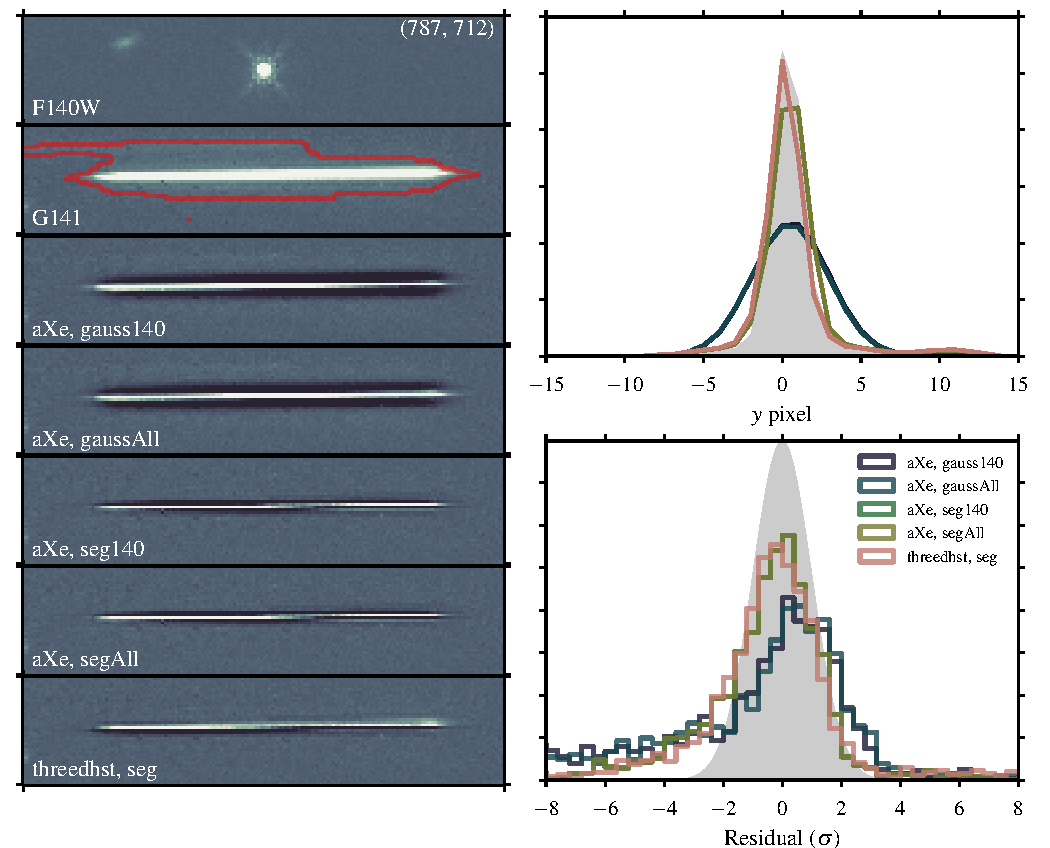
\includegraphics[scale=0.9, angle=0.0]{Figures/compare_model_star.pdf}
    \caption{2D spectrum of a star.  The top panel shows the F140W image offset to put the object at the center of the panel.  The second panel shows the observed G141 spectrum.  The red outline shows the subset of pixels used in the distribution of residuals shown in the lower right panel.  The bottom five 2D spectrum panels show the $observed-model$ residuals for the modeling codes and input assumptions, as labeled.  The top right panel shows the spatial profile of the 2D spectrum collapsed along the $x$ (wavelength) axis for the observed (filled gray) and model (colored lines) spectra.}
    \label{fig:star2D}
\end{figure}

\begin{figure}
    %\epsscale{1.0}
    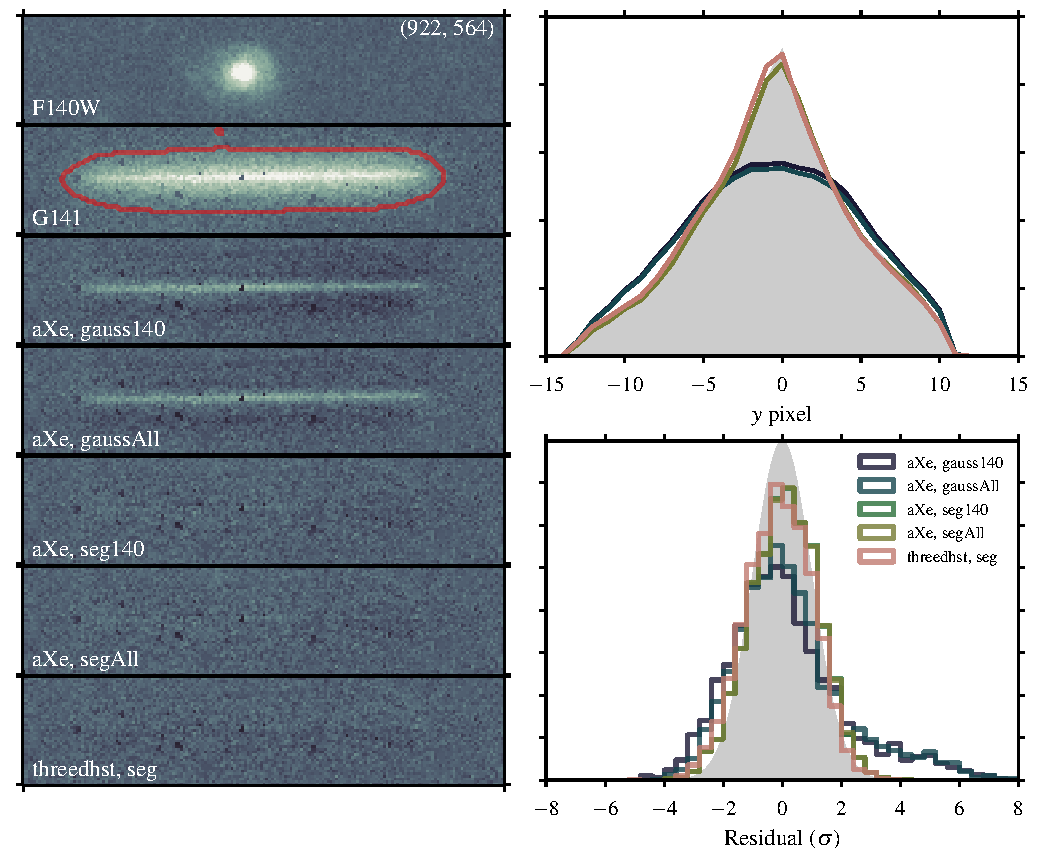
\includegraphics[scale=0.9, angle=0.0]{Figures/compare_model_galaxy3.pdf}
    \caption{2D spectrum of an extended galaxy.  The panels are the same as Fig.~\ref{fig:gal2D}.  The fit residuals are somewhat better than for the stellar model because PSF and discrete pixel grid effects are less important for the extended galaxy.}
    \label{fig:gal2D}
\end{figure}

\ssection{A Comment on Next Generation Grism Analysis Software}\label{sec:nextgen} 
% this paragraph was written by RER on Oct 13, 2014.

A key limitation to the methods presented above is dealing with deblending (or contamination) of overlapping spectra and optimally combining information from multiple orientations or positions.  
While \texttt{aXe} uses the same engine as \texttt{aXeSIM} to quantitatively estimates the amount of spectral contamination, this information is not used to deblend, or clean, calibrated spectra. This information is instead provided solely as a (fixed) quantitative estimate of the contamination. At present, the WFC3 Grism Group is exploring two different (but related) methods based on their computational feasibility, fundamental assumptions, and limiting systematics.  The first method, {\it forward modeling}, essentially seeks to predict a given dispersed image based on the properties of the sources (such as number/position of sources and their spectra).  These properties are optimized by comparing with the observed dispersed image, but typically the positions are held fixed (to those seen in the direct image).  The second method, {\it linear reconstruction}, attempts to reconstruct the optimal spectra by inversion using least-squares techniques.  Each approach has unique pros and cons, and neither seems to be inherently superior at this stage.  We have just begun developing prototypes of these tools which are not necessarily built using previously discussed pipelines or configurations, indeed we leave open the possibility that new calibrations, reference files, or descriptions of the grism images will be needed for these tools.  


\newpage

\appendix

\ssection{The aXe Configuration File}\label{sec:axeconf}
\texttt{aXe}, \texttt{aXeSIM}, \texttt{NPspec} and \texttt{threedsht} rely on an \texttt{aXe} configuration file to describe how to simulate and extract \textit{HST} slitless spectra. The \texttt{aXe} configuration file is based on the assumption that every aspect of the instrument calibration can be parametrized as $n^{th}$\ order polynomial. The field dependence (how the dispersion varies across the detector) is also assumed to be smooth varying and to be approximated as a 2D polynomial function of the $m^{th}$\ order. While multiple orders are treated independently in a single \texttt{aXe} configuration file, a separate \texttt{aXe} configuration file is required for each detector of each instrument. The two WFC detectors on the ACS instrument, for example, are treated independently. Overlaps bettween multiple detectors of an instrument is not usually a problem as the dispersion is in the $x$-direction while the detectors are stacked in the $y$-direction. \texttt{aXe} does not attempt to combine spectra obtained using both detectors, for example when large dithers in the $y$-direction are used.

For the purpose of simulations, the \texttt{aXe} configuration file is used to identify the various spectral orders to be simulated (which are referred as ``BEAMs'' in the \texttt{aXe} configuration file). For a given order (beam ``A'' is usually associated with the brightest $+1^{st}$\ order), there are two parameters of interest: DYDX and DLDP. They describe the spectral trace and its wavelength dependence, respectively. DYDX produces the expected offset $dy$ in the $y$-direction with respect to the $y$-position of the source (as measured through an imaging filter without the dispersing element) as a function of $dx$, the offset between source and a given column in the $x$-direction:
\begin{dmath}
dy = a_0 + a_1 \cdot dx + a_2 \cdot dx^2 + ... + a_n \cdot dx^n, \label{eq:1}
\end{dmath}
where $dy$\ is the offset (in pixels) between the centroid of the trace and the $y$ position (pixel~$j$) of the source, $dx$\ is the offset in the $x$-direction between a particular pixel on the trace and the $x$-position (pixel~$i$) of the source (Figure~\ref{fig:trace}). The order of the polynomial is $n$, with $n=1$ corresponding to a simple linear dispersion. If the instrument had no field dependence and dispersed all spectra in the same way across the field of view, the coefficients $a_n$ would be simple constants. In the case of WFC3, however, there is a significant amount of field dependence of the trace and this is parametrized by allowing each value of $a_n$ to itself be a 2D polynomial that is a function of the source position ($i$,$j$) on the detector.  In the case of a second order 2D field dependence, we have
\begin{dmath}
a_n(i,j) = b_{n,0} + b_{n,1} \cdot i + b_{n,2} \cdot j + b_{n,3} \cdot i^2 + b_{n,4} \cdot i \cdot j + b_{n,5} \cdot j^2. \label{eq:2}
\end{dmath}
A second order 2D field dependent representation of a linear ($n=1$) dispersion therefore becomes
\begin{dmath}
dy(i,j,dx) = b_{0,0} + b_{0,1} \cdot i + b_{0,2} \cdot j + b_{0,3} \cdot i^2 + b_{0,4} \cdot i \cdot j + b_{0,5} \cdot j^2 + dx~(b_{1,0} + b_{1,1} \cdot i + b_{1,2} \cdot j + b_{1,3} \cdot i^2 + b_{1,4} \cdot i \cdot j + b_{1,5} \cdot j^2), \label{eq:3}
\end{dmath}
where we have explicitly expressed $dy$ as a function of the source position ($i$,$j$) and of the $x$-offset ($dx$) between the source and a particular point on the spectrum.

\begin{figure}[!t]
\centering
\includegraphics[width=6.5in]{"Figures/trace_fig"}
\caption{The slitless trace. The object, as it would be visible using a broad band filter, is shown at the bottom left and has pixel coordinates of ($i$,$j$). We also show on the same Figure the resulting spectrum as produced by the G141 grism. The measurements quantities $dx$ and $dy$ used in Equations \ref{eq:1}, \ref{eq:2} and \ref{eq:3} are shown.}
\label{fig:trace}
\end{figure}

\begin{figure}[!t]
\centering
\includegraphics[width=6.5in]{"Figures/wave_fig"}
\caption{The wavelength calibration. The wavelength along the trace is computed as a function of the dp, the arc along the trace from the reference pixel (point on the trace with the same x-coordinate as the reference pixel) and a given position on the trace.}
\label{fig:wave}
\end{figure}

The description of the wavelength dependence {\em along} the trace DLDP is similar and parametrizes the difference in wavelength between the reference point on the trace and a given position on the trace.
\begin{dmath}\label{eqn:lam}
\lambda = \alpha_0 + \alpha_1 \cdot dp + \alpha_2 \cdot dp^2 + ... + \alpha_n \cdot dp^n \label{eq:4}
\end{dmath}
where again, a 2D field dependence implies
\begin{dmath}
\alpha_n(i,j) = \beta_{n,0} + \beta_{n,1} \cdot i + \beta_{n,2} \cdot j + \beta_{n,3} \cdot i^2 + \beta_{n,4} \cdot i \cdot j + \beta_{n,5} \cdot j^2 \label{eq:5}
\end{dmath}
and we have, in the case of a linear wavelength dispersion solution,
\begin{dmath}
\lambda(i,j,dp) = \beta_{0,0} + \beta_{0,1} \cdot i + \beta_{0,2} \cdot j + \beta_{0,3} \cdot i^2 + \beta_{0,4} \cdot i \cdot j + \beta_{0,5} \cdot j^2 + dp~(\beta_{1,0} + \beta_{1,1} \cdot i + \beta_{1,2} \cdot j + \beta_{1,3} \cdot i^2 + \beta_{1,4} \cdot i \cdot j + \beta_{1,5} \cdot j^2) \label{eq:6}
\end{dmath}

The \texttt{aXe} configuration file encodes the $b_{n,m}$\ parameters of Equation \ref{eq:3} (describing the trace) in DYDX and the $\beta_{n,m}$\ parameters of Equation \ref{eq:6} (describing the wavelength dispersion) in DLDP.  To be precise, $dp$ in the preceding equations is the arc-length along the trace, given as:

\begin{dmath}
dp(X) = \int_{0}^{X} \sqrt{1+y'(x)^2}\, dx
\label{eq:dldp}
\end{dmath}
where $y'(x) = dy/dx$.  For $n\leq2$, this integral has analytic solutions, which we 
utilize in the example code below.  For higher order $dy/dx$ trace shapes, such as the curved orders of the WFC3/UVIS G280 grism, we evaluate this integral numerically (which 
can be very slow).

\ssection{Code to compute the spectral trace}\label{sec:examplecode}
%\lstlistoflistings
%\newpage
We provide the Python code below to demonstrate reading the \texttt{aXe}-formatted configuration files and computing the spatially-dependent dispersion parameters DYDX and DLDP (\S\ref{sec:axeconf}).  Updates to the code (and updates to this document itself) can be found at: 
\begin{center}
\url{https://github.com/WFC3Grism/CodeDescription/}.
\end{center}

\lstinputlisting[language=Python]{grism.py}




\end{document}